\chapter{Исследование}

\section{Технические характеристики}
Характеристики используемого оборудования:
\begin{itemize}
    \item[---] операционная система --- Windows 11 Home~\cite{windows};
    \item[---] память --- 16 Гб;
    \item[---] процессор --- 12th Gen Intel(R) Core(TM) $i7-12700H$ @  2.30 ГГц~\cite{intel}.
\end{itemize}

\section{Описание исследования}

Во время выполнения, в программе фиксируются моменты времени начала и конца обработки рецепта очередным этапом конвейера. Простои обработчиков можно увидеть на рисунке~\ref{fig:plot}.

\begin{figure}[h]
	\centering
	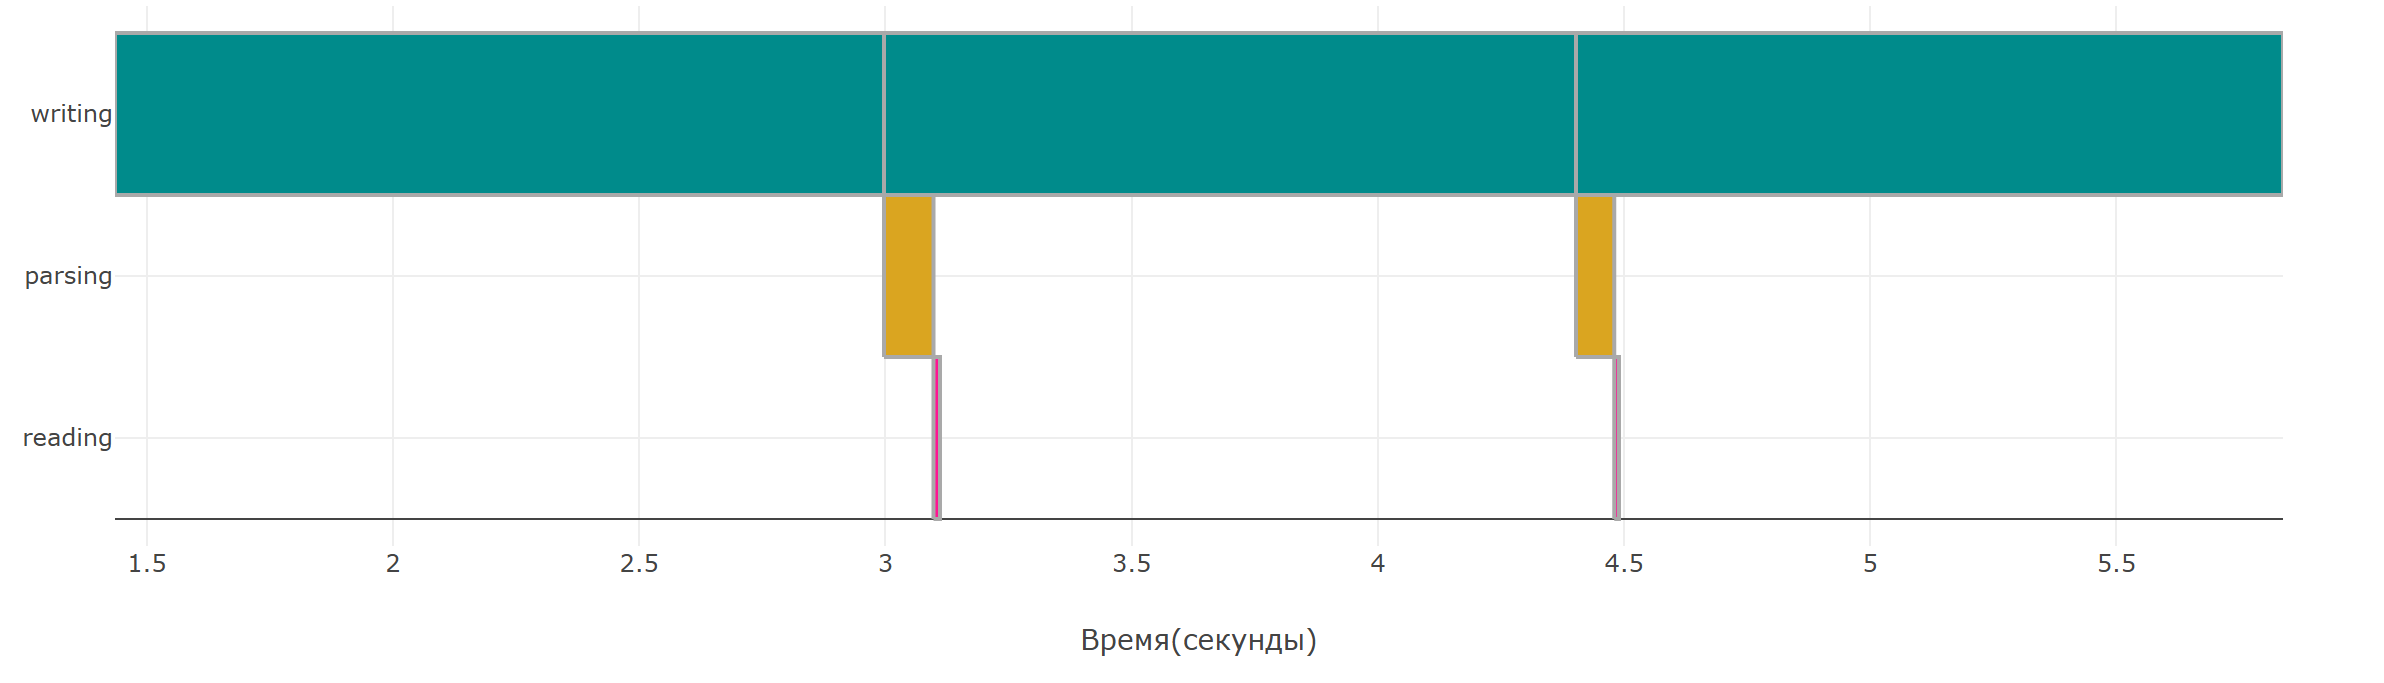
\includegraphics[width=0.8\textwidth]{images/plot.png}
	\caption{График зависимости времени выполнения от количества страниц}
	\label{fig:plot}
\end{figure}

\clearpage

Суммарное время простоя и работы каждого этапа представлено на таблице~\ref{tbl:mes}.

\begin{table}[h]
    \begin{center}
        \begin{threeparttable}
    \caption{Описание тестовых случаев}
    \captionsetup{justification=raggedright, singlelinecheck=false}
    \label{tbl:mes}
    \begin{tabular}{|c|r|r|}
        \hline
        \textbf{Название этапа} & \textbf{Среднее время работы(с)} & \textbf{Среднее время простоя(с)} \\
        \hline
        reading & 1.6131 & 0.0000 \\
        \hline
        parsing & 0.0873 & 1.6392 \\
        \hline
        writing & 0.0106 & 1.7123 \\
        \hline
    \end{tabular}
    \end{threeparttable}
    \end{center}
\end{table}

В результате исследования было получено, что при выполнении параллельных вычислений в конвейере возможны простои отдельных его частей. Это означает, что в определенные моменты времени часть конвейера может простаивать, ожидая поступления данных от предыдущих этапов обработки.

\clearpage